% \documentclass{article}
\documentclass[journal]{IEEEtran}
% \usepackage[margin=1in]{geometry}
\usepackage[hidelinks]{hyperref}
\usepackage{verbatim}
\usepackage{amsmath}
\usepackage{graphicx}
\usepackage{minted}
\usepackage{subcaption}
\usepackage{booktabs}

\setminted{fontsize=\footnotesize, tabsize=2, breaklines=true}

% \newcommand{\ttfont}[1]{{\fontfamily{cmtt}\selectfont #1}}

\title{picoDAW: a web-based sequencer/synthesizer/sampler}
\author{
	Tim Fan (SID: 550790019) \\
	fanchenhao2206 \\
	\texttt{repo: \url{https://github.com/fanchenhao2206/elec5305-project-550790019}}\\
	\texttt{site: \url{https://fanchenhao2206.github.io/elec5305-project-550790019}}
}

\begin{document}

\maketitle

\section{Project Overview}

\begin{comment}
3. Project Overview
Briefly describe the goal of your project. Include:
• The problem you are addressing
• Why it is important
• Your proposed solution
Example: This project aims to develop a real-time noise suppression algorithm for 
mobile devices using a lightweight neural network. The goal is to improve speech 
intelligibility in noisy environments.
\end{comment}

This project aims to develop a synthesizer and sequencer---aka a digital audio workstation (DAW)---for any device capable of running a modern web browser supporting WebAudio, using the emscripten compiler toolchain 
that turns C++ DSP code into efficient WebAssembly.
The goal is to make sound and music production more accessible, because any device capable of running 
a modern web browser will be able to use this DAW, not just computers or tablets running OS-dependent 
and discrete, native DAW applications.

\section{Definitions}

\noindent
Before moving on, I want to briefly describe what I mean by a sequencer/synthesizer/sampler, 
and also what a digital audio workstation---aka DAW---is. 

\subsection{Synthesizer}
\noindent
What I mean by a synthesizer instrument, is something that generates and plays a sound---creates audio-frequency
air pressure waves---on demand. So, when you press a key on the synthesizer's input controller, the 
synthesizer will generate---aka synthesize---and play a sound, corresponding to what key was pressed. For 
example, a basic sawtooth synthesizer is a synthesizer that creates the sawtooth wave sound on demand, 
its frequency---aka pitch---depending on which key is played on the keyboard connected to it. Pressing the 
key corresponding to the pitch A5, will result in the synthesizer synthesizing and playing a sawtooth 
wave sound at 880Hz. 

\subsection{Sampler}
\noindent
A sampler instrument, in my understanding, is actually very similar, except that instead of generating a new sound, 
it will take an existing sound---e.g. the wave format recording of a real-life snare drum being hit---and 
play it back on demand; possibly also modifying or processing it before playing it back. For example, pressing 
one key might play back the snare drum recording in its original form, literally re-playing the original wave 
recording. While pressing another key might play back the recording at half its sample rate, resulting in 
the same sound but lowered one octave.

\subsection{Sequencer}
\noindent
At the core of both these instruments are their respective input controllers; 
typically used by the human body, whether that be through hitting it, blowing air into it, stepping on it, etc.
The sequencer then, in my understanding, gets its name from the idea from an instrument that can be played, not by 
hitting it directly, but by providing it a sequence of instructions on what keys the instrument should press for 
itself, and when and in what order.

An example of such an instrument is the player piano\footnote{\url{https://en.wikipedia.org/wiki/Player_piano}},
which reads the desired keys to be pressed from a sheet of paper, written by a human who punches holes in the paper 
corresponding to the keys they want the instrument to press, and when they should be pressed. In essense, like how 
early computers were programmed, through punch cards. Presumably, because the sheets of player piano paper could get 
very long, they would be rolled up, giving them their name; piano rolls\footnote{\url{https://en.wikipedia.org/wiki/Piano_roll}}. 

A sequencer then, in my understanding, is the machine a human would use to write the program---e.g. 
a piano roll---that will then be loaded by an instrument that can understand this program; in this 
case, a player piano.
Perhaps the most common type of sequencer, fittingly, is based off the piano roll. In REAPER\footnote{\url{https://www.reaper.fm}} 
for example, the ``piano roll'' mode of its sequencer is the default mode (fig. \ref{fig:reaper_piano_roll}). 
Other modes include the ``musical notation'' mode, which is based off the Western Art or classical 
music tradition of sheet music (fig. \ref{fig:reaper_music_notation}).

\subsection{Digital audio workstation}
\noindent
A typical DAW then, is an application that combines all of the above---sequencer/synthesizer/sampler---alongside 
many other features useful for professionals and experienced hobbyists. 
For example, a DAW like the aforementioned REAPER will also allow you to record audio through it; the 
recording can then of course be played back though its sampler. Note that because the sampler is also an 
instrument, the timing of playback can also be sequenced through the included sequencer. And, though 
it comes with pre-installed instruments, third-party instruments can also be used with its sequencer, 
through integration with software instrument standards like the VST\footnote{\url{https://en.wikipedia.org/wiki/Virtual_Studio_Technology}}.

\begin{figure}[t]
	\centering
	\begin{subfigure}[b]{0.48\columnwidth}
		\centering
		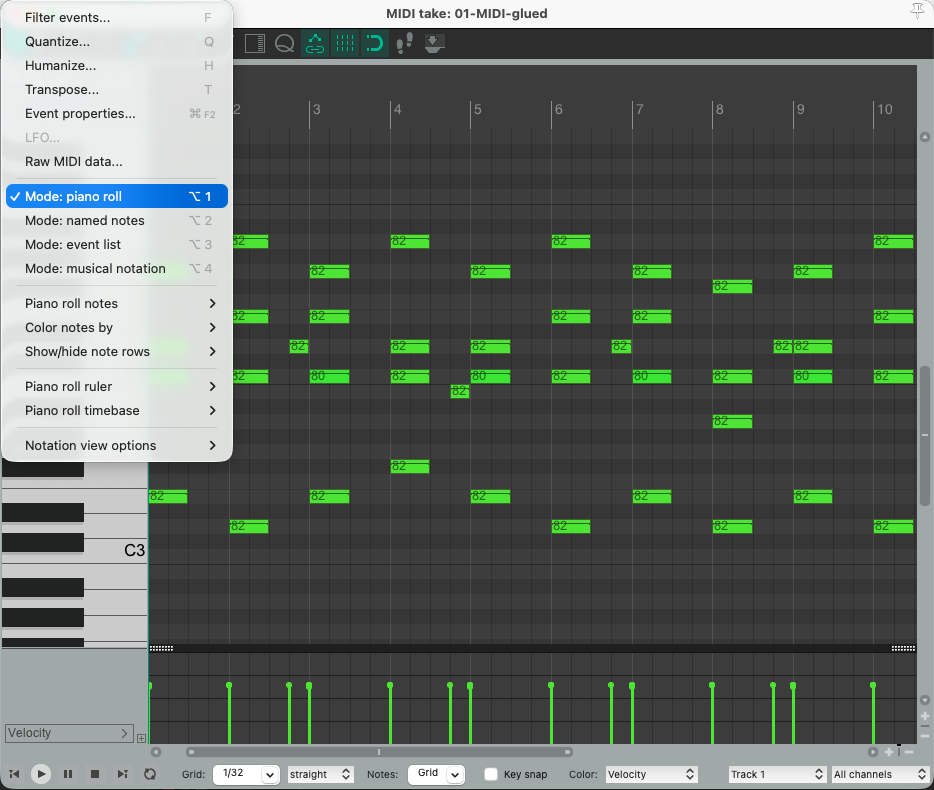
\includegraphics[width=\linewidth]{images/reaper-piano-roll}
		\caption{Piano Roll}
		\label{fig:reaper_piano_roll}
	\end{subfigure}
	\hfill
	\begin{subfigure}[b]{0.48\columnwidth}
		\centering
		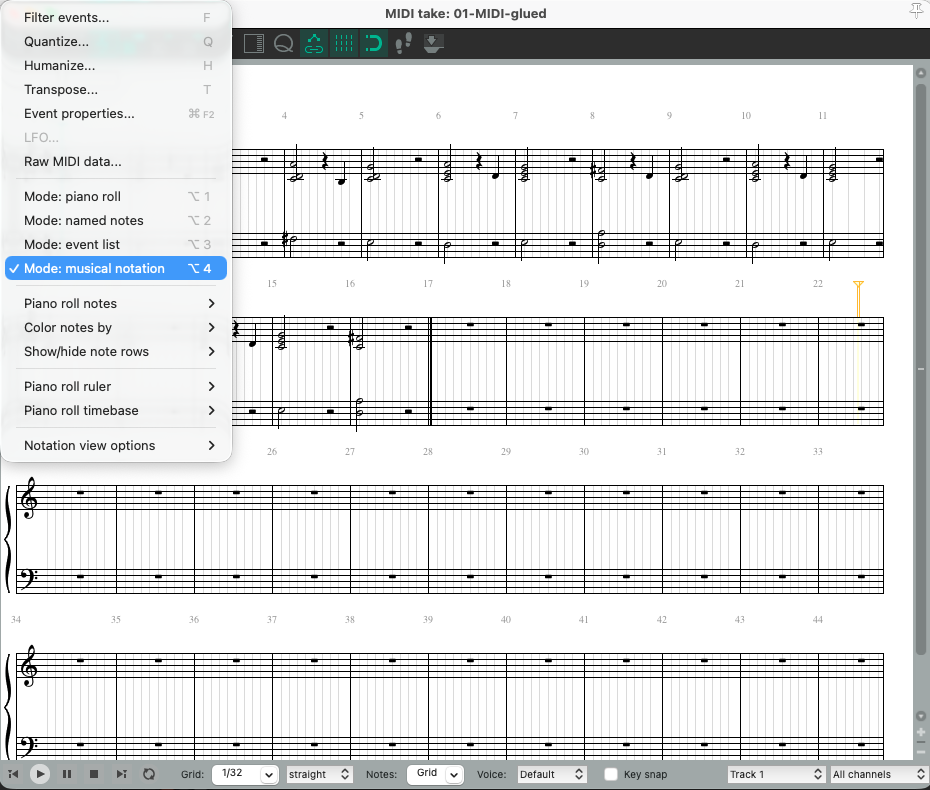
\includegraphics[width=\linewidth]{images/reaper-musical-notation}
		\caption{Musical Notation}
		\label{fig:reaper_music_notation}
	\end{subfigure}
	\caption{The modes of REAPER's MIDI sequencer}
\end{figure}


\section{Background and Motivation}

\begin{comment}
Provide context and motivation for your project.
• What existing solutions or research are relevant?
• Why did you choose this topic?
Example: Recent advances in deep learning have enabled effective noise suppression, but many
models are too large for mobile deployment. This project explores efficient architectures suitable
for embedded systems
\end{comment}

\noindent
Despite its relatively recent history, with the first publication of a working draft in only 
2011\footnote{\url{https://www.w3.org/TR/2011/WD-webaudio-20111215/}}, the WebAudio API has seen 
extensive development over the course of a decade, eventually receiving an endorsement from the W3C 
in 2021 as a Recommendation\footnote{\url{https://www.w3.org/TR/webaudio-1.0/}}. Notably, its primary 
\texttt{AudioContext} interface has been fully supported by most major web browsers since at least 
2015\footnote{\url{https://developer.mozilla.org/en-US/docs/Web/API/Web_Audio_API\#browser_compatibility}},
with the only exception being Safari which implemented support in 
2021\footnote{\url{https://developer.apple.com/documentation/safari-release-notes/safari-14_1-release-notes\#WebKit-Framework}}.

Of course, audio has existed for a much longer time than that on the internet. As Boris Smus describes 
in their brief history of audio on the web \cite{boris_smus}, initially that was through the Flash external 
plugin for browsers, and then later through the HTML5 \texttt{<audio>} element which was instead natively 
supported by the web browser itself. In fact, it's this \texttt{<audio>} element that allows music 
streaming websites like Bandcamp to preview an artist's music through the web browser 
(see Fig. \ref{fig:wanderstop}).

\begin{figure}[!htbp]
	\centering
	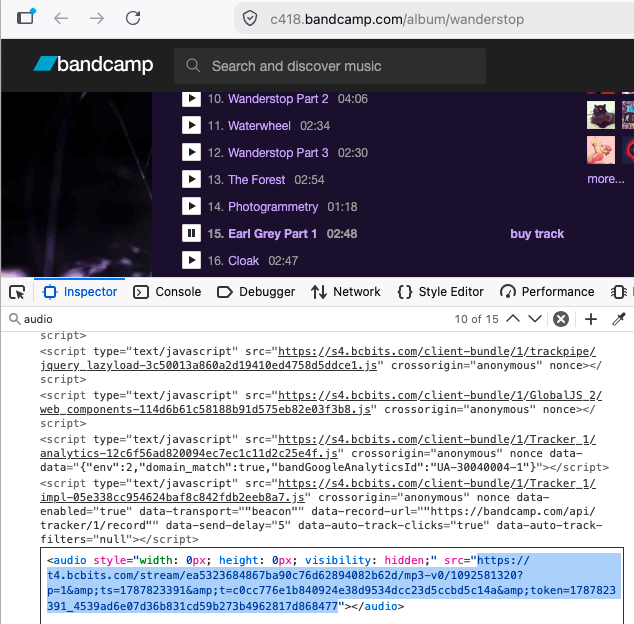
\includegraphics[width=0.6\columnwidth]{images/wanderstop-0}
	
	\texttt{Input ... from `1092581320.mp3' Duration: 00:02:48.00, ..., bitrate: 236 kb/s}

	\caption{Bandcamp allows artists to offer their listeners a compressed and lower bitrate MP3 preview of their tracks, played in the browser through the HTML5 \texttt{<audio>} element. The text above is the result of \texttt{ffprobe 1092581320.mp3}}
	\label{fig:wanderstop}
\end{figure}

But one thing Flash's plugin did for web audio that HTML5's \texttt{<audio>} element doesn't do, is 
allow for interactive audio. For example, a synthesizer/sampler/sequencer like the one this project 
will aim to build, would require a predictable amount of latency between a person pressing a key on 
their keyboard and the corresponding sound being played through their speakers, something that the 
\texttt{<audio>} element just wasn't designed for.

\begin{comment}
Instead, it was designed for cases like Bandcamp's 
song previews, where a one second delay between pressing to pause a song and the song actually pausing,
though annoying, is ultimately benign and would likely be fixed by restarting the browser. But for a real
time instrument like a web synthesizer? That would be incredibly disorientating for a live performance; 
having to wait one second to hear the note they want to play would make the instrument virtually 
unusable.
\end{comment}

That is the kind of problem the WebAudio API attempts to solve, and why it has been possible for 
synthesizers and other real time instruments to be built for the web. For example stevengoldberg's 
emulation of the Juno-106 synthesizer\footnote{\url{https://github.com/stevengoldberg/juno106}} 
built for the web in 2015, to ryukau's collection of 
synthesizers\footnote{\url{https://github.com/ryukau/UhhyouWebSynthesizers}} build for the web which 
use the aforementioned \texttt{AudioContext} interface as the backbone of its audio framework 
(see Fig. \ref{fig:ryukau}).

\begin{figure}[!hbtp]
\begin{minted}{javascript}
// Copyright Takamitsu Endo (ryukau@gmail.com)
// SPDX-License-Identifier: Apache-2.0

export class Audio {
  cachedBuffer = null;
  constructor() {
  	// Initialise AudioContext
    this.audioContext = new AudioContext();
  }
  play() {
    // If no AudioBuffer
    if (!this.cachedBuffer) {
      // Create AudioBuffer object
      let buffer = this.audioContext.createBuffer(
        this.audioContext.sampleRate);
      for (let i = 0; i < this.wave.channels; ++i) {
        // Write to AudioBuffer
        buffer.copyToChannel(new Float32Array(
          this.wave.data[i]), i, 0);
      }
      this.cachedBuffer = buffer;
    }
    // And set AudioContext's AudioBuffer to our's
    this.source = 
      this.audioContext.createBufferSource();
    this.source.buffer = cachedBuffer;

    // And play
    this.source.start();
  }
}
\end{minted}
\caption{Heavily redacted version of the custom Audio class used by ryukau\textsuperscript{6} at 
\texttt{common/wave.js} which uses the WebAudio API}
\label{fig:ryukau}
\end{figure}


\section{Proposed Methodology}

\begin{comment}
which I argue does not necessarily make 
it any more accessible or approachable than its native counterparts. 

Another example are web-based grooveboxes TODO TODO

GROOVEBOX (pads, things like that)

Thus, this project argues the need for a 
web-based DAW-like application, that at the same time does not resemble the traditional fully-featured
desktop-based DAW it shares the same name with.

DS-10

So this gets to the core of this proposal; what design would meet the goal I have set out to achieve? 
My proposal is the DS-10; a clone of it.
\end{comment}

\noindent
proposal

\section{Expected Outcomes}

\begin{comment}
Describe what you expect to deliver:
• A working prototype or simulation
• Performance metrics (e.g., signal-to-noise ratio (SNR) improvement, Perceptual Evaluation
of Speech Quality (PESQ) score)
• GitHub documentation and demonstration
\end{comment}
\noindent
Of course, the ultimate deliverable will be a working prototype of picoDAW deployed onto the 
provided GitHub project site. Given the complexity of a DAW however---even a stripped down 
one, only a sequencer/synthesizer/sampler---the core mantra behind the project will be to 
keep it simple, stupid. 

This means, the UI will be basic without the polish of the actual 
DS-10 it'll take inspiration from. Furthermore, though audio effects like real-time reverb 
or delay, and features like a semi-modular patchbay, are incredibly useful in modern music 
creation, they will not be prioritised over a working prototype.

What is a non-negotiable 
though, is the inclusion of a low pass and high pass filter for each instrument, 
and an envelope to control its cutoff frequency; alongside a second envelope for volume. In summary,
the expected features will be a:
\begin{enumerate}
	\item Synthesizer and sampler as instruments
		\begin{itemize}
		\item 4 Synthesizers; each has sine, saw, triangle, square, and noise as possible oscillator options
		\item 2 Samplers; each can load a \texttt{.wav} sample from 0.1 to 1 second, resampled to 48kHz on upload
		\end{itemize}
	\item Step sequencer with 16 steps. At a default 120bpm, this means only 8 seconds of audio, played in a loop
		\begin{itemize}
		\item The 6 instruments will each have their own
		\item The sequencer will have two screens
			\begin{itemize}
			\item one for sequencing what key is pressed and when
			\item one for how long that key should be pressed
			\end{itemize}
		termed Note and Gate respectively on the DS-10
		\item Changes to pattern during play will reflect on loop
		\end{itemize}
	\item Filter with adjustable cutoff and peak/resonance, toggled between lowpass and highpass.
		\begin{itemize}
		\item The 6 instruments will each have their own filter
		\end{itemize}
	\item ADSR\footnote{\url{https://en.wikipedia.org/wiki/Envelope_(music)\#ADSR}} envelope
		\begin{itemize}
		\item The 6 instruments will each have two envelopes
			\begin{itemize}
			\item one for modulating the cutoff of its filter
			\item one for modulating the volume of its output
			\end{itemize}
		\end{itemize}
	\item Mixer
		\begin{itemize}
		\item Basic; toggle mute or solo for each instrument
		\end{itemize}
\end{enumerate}

\begin{figure}[!hbtp]
	\centering
	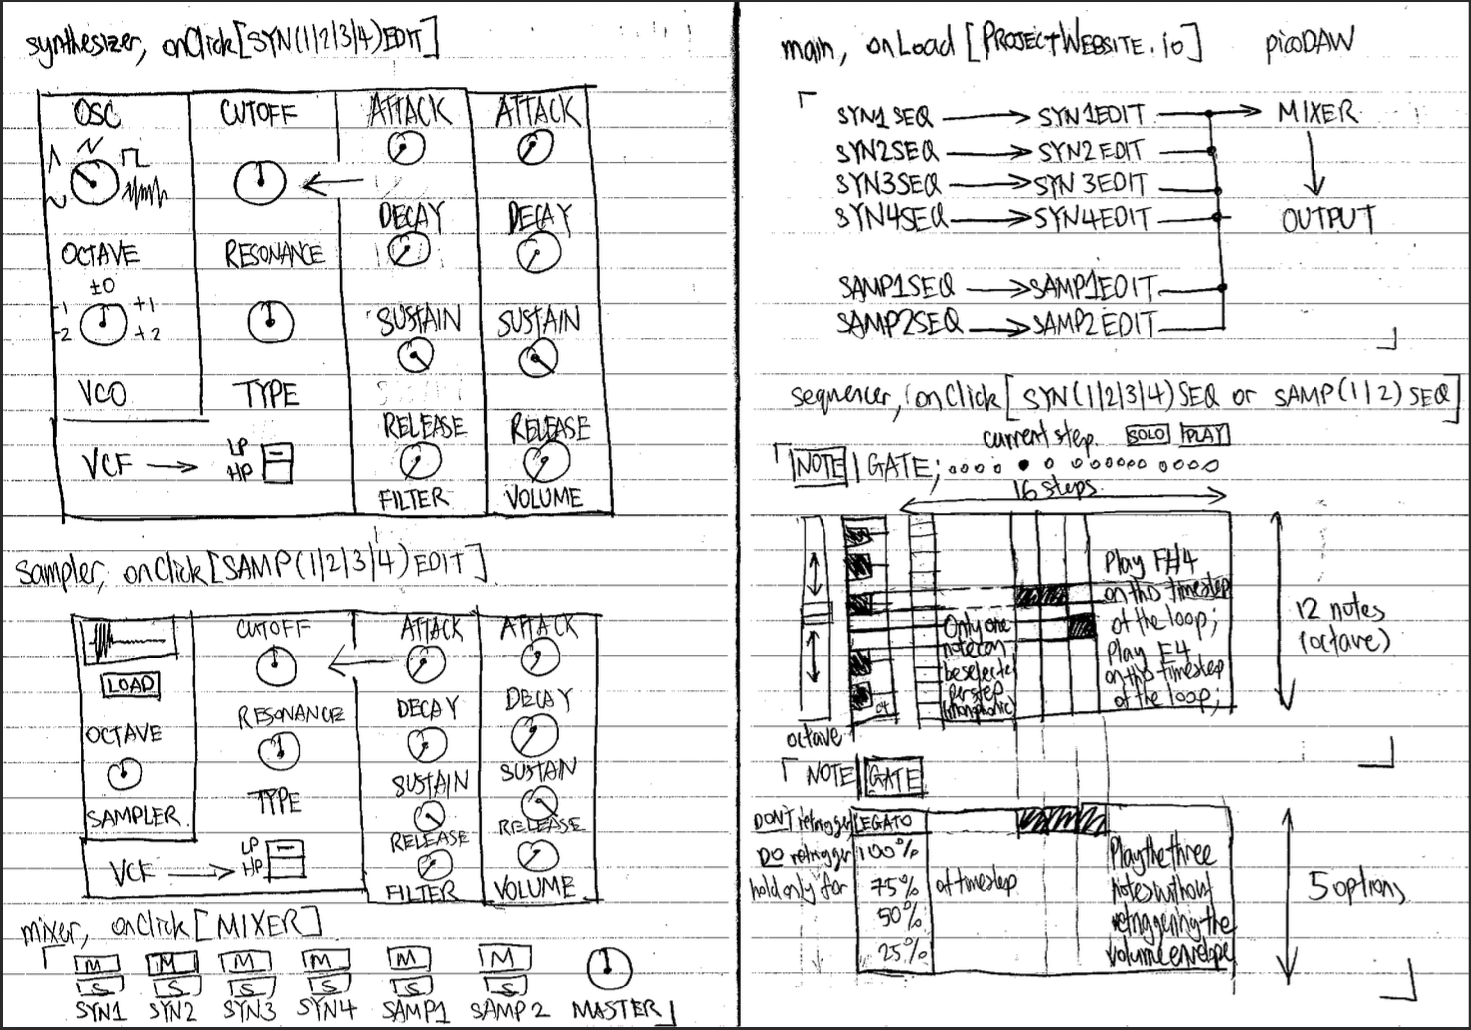
\includegraphics[width=0.9\columnwidth]{images/draft}

	\caption{Draft mockup of UI for picoDAW}
	\label{fig:draft}
\end{figure}
\noindent
See fig. \ref{fig:draft} for a draft mockup of picoDAW's UI.

Stretch goals, in case development goes easier than expected, include: (i) Pattern sequencer, enabling 
more expressive song creation; build multiple patterns, and then sequence them together to create a 
song. (ii) Two oscillators per synthesizer---instead of just one---making it easier to create chords, 
since the pitch of the second oscillator could be tuned to a specific note above or below the first 
oscillator. (iii) Volume control in mixer for each instrument, and basic effects---reverb, delay, and 
EQ---with routing done through the mixer. (iv) One 
LFO\footnote{\url{https://en.wikipedia.org/wiki/Low-frequency_oscillation}} per instrument; a triangle 
oscillator---of low frequency, proportional to \texttt{1/base\_timestep}---whose output can modulate 
the pitch of the instrument, providing basic FM synthesis. 




\section{Timeline}

\begin{comment}
Weeks 1-4   Considered Project Topic
Weeks 5-6   Implement sequencer to trigger sine synth on note wrt. gate values
            This includes an ADSR envelope for volume
Weeks 7-8   Implement synths; lowpass and highpass filter with ADSR envelope too
            Try implement sampler too; hopefully a lot of everything is code reuse
Weeks 9-10  Implement mixer; code refactoring to prepare for report/submission
Weeks 11-13 Report writing, prototype cleanup, extra features if meet stretch goal
\end{comment}

\begin{table}[!hbt]
	\centering
	\renewcommand{\arraystretch}{1.2}
	\begin{tabular}{c p{0.72\columnwidth}}
		\toprule
		\textbf{Week} & \textbf{Task} \\
		\midrule
		1--4 & Considered project topic; research and literature review \\
		5--6 & Implement sequencer to trigger included sine synth wrt. volume envelope; on notes and following gate values\\
		7--8 & Setup testing framework; implement low-pass/high-pass filters with envelopes on their cutoff frequencies \\
		9--10 & Implement additional oscillators, sampler, and mixer; refactor system to maximise code reuse\\
		11--13 & Report writing; bug fixes, implementation of extra features if stretch goals are met, prototype cleanup \\
		\bottomrule
	\end{tabular}
\end{table}


\bibliographystyle{IEEEtran}
\bibliography{references}

\end{document}
